\section{Skip Lists}

\subsection{Skip List vs. Ordered Map}

\begin{tcolorbox}[title=Disclaimer]
	The implementation of the skip list is nowhere near the level of polish the built-in ordered map has. Thus, it is expected to perform worse. (I'm just not motivated enough to learn C++) Thus, I think this portion will be more like a study of the pattern of the latency as more elements are added to it in the skip list. The implementation of the skip list can be found \href{https://github.com/nngerncham/cs315_apal/tree/main/assignments/asn01/03-skip-list}{here}.
\end{tcolorbox}

\subsubsection{Insert Latency}
\begin{figure}[H]
	\begin{center}
		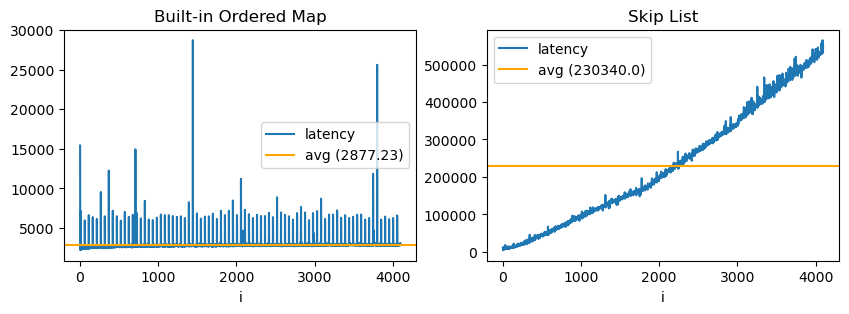
\includegraphics[width=0.9\textwidth]{03-insert-latencies.png}
		\caption{Insert latency of a C++ built-in ordered map and a skip-list}
		\label{fig:03-insert-latency}
	\end{center}
\end{figure}

From some inspection of my own code, I've come to a realization that the insertion method is very poorly optimized as it needs to go through each level at least half the time in order to insert the new node in, making its performance horrendous. This doesn't need analysis, \textit{this needs to be rewritten} (but I'm out of motivation).

\begingroup

\subsubsection{Search Latency}
\begin{figure}[H]
	\begin{center}
		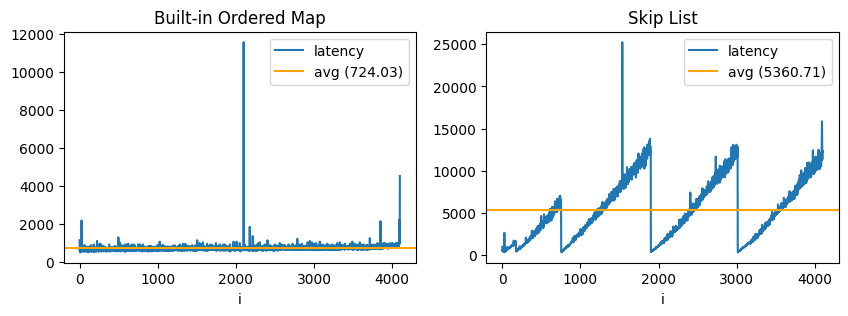
\includegraphics[width=0.9\textwidth]{03-search-latencies}
		\caption{Search (get) latency of a C++ built-in ordered map and a skip-list}
		\label{fig:03-search-latency}
	\end{center}
\end{figure}

\begin{wrapfigure}{l}{0.4\textwidth}
	\centering
	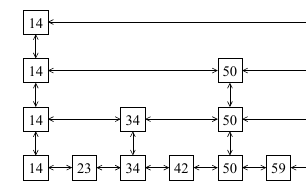
\includegraphics[width=0.4\textwidth]{03-lecture-note-sl.png}
	\caption{Skip list diagram from lecture note}
\end{wrapfigure}

Here is an interesting case of \textit{I'm not sure what is going on}.
However, we might be able to learn something about how the skip list search works since there is a pattern in the latency.

From the plot, we can infer that the access pattern is as follows. There are some elements that is reachable from the top level, so it takes very minimal time to reach. Then, there are roughly about the same number of elements that are reachable from the second highest level. This pattern continues on to form a staircase-like structure which what we have observed from the plot. This coincides with the visualization of the skip list seen in class and the original paper.

\endgroup

\subsubsection{Delete Latency}
\begin{figure}[H]
	\begin{center}
		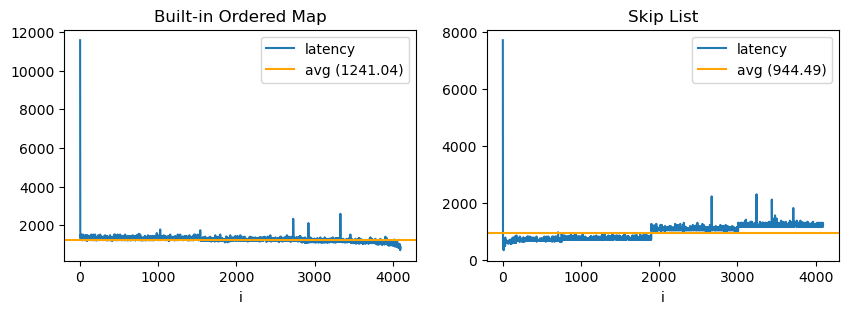
\includegraphics[width=0.9\textwidth]{03-delete-latencies.png}
		\caption{Delete latency of a C++ built-in ordered map and a skip-list}
		\label{fig:03-delete-latency}
	\end{center}
\end{figure}

Here is the only case that the skip list `outperforms' the ordered map, but that could be simply left to the margin of error in latency measurement. Assuming that the ordered map is implemented with a balanced binary search tree, the running time should be the same as in both data structure algorithm-wise as they, in the worst case, need to go through every level of the tree/list. Therefore, it is expected that they perform roughly about the same.

\subsection{Better Search Algorithm}

With the assumption that we can go up and down between each levels of the skip list with minor modification to the original, a more efficient search algorithm goes as follows.

\begin{algorithm}
\caption{Search algorithm for key $k$ in skip list $L$}
\begin{algorithmic}[1]
\Procedure{Search}{$k, L$}
	\State $V \gets$ Node with smallest key in $L$
	\While {$V_\text{next$\to$key} < k$} \Comment{Goes up to the highest level with max key less than $k$}
		\While {$V_\text{above} \neq \text{NULL} \cap V_\text{above$\to$next$\to$key} < k$}
			\State $V \gets V_\text{above}$
		\EndWhile
		\State $V \gets V_\text{next}$
	\EndWhile
	\While {$V_\text{below} \neq$ NULL} \Comment{Goes down to the bottom level}
		\State $V \gets V_\text{below}$
		\While {$V_\text{next$\to$key} < k$}
			\State $V \gets V_\text{next}$
		\EndWhile
	\EndWhile
	\If {$V_\text{key} = k$}
		\State \Return Success
	\Else
		\State \Return Failure
	\EndIf
\EndProcedure
\end{algorithmic}
\end{algorithm}

\subsubsection{Running Time Analysis}

\begin{tcolorbox}
\textbf{Lemma.} Given a key $k$, there are $O(\log d)$ valid levels with high probability where $d$ is the number of elements whose key is smaller $k$.
Here, a valid level refers to levels with at least one node $v$ where $v_\text{next$\to$key} < d$ or $v$ points to a node whose key is still less than $d$.

\textbf{Proof.} Given some key $k$, consider the element $e_k$ with key $k$. The probability of $e_k$ showing up in more than $c\log d$ levels is $1/2^{c\log d} = 1/d^c$.
As for the rest of the elements smaller than it, the probability of the remaining $d$ elements having more than $c\log d$ levels is bounded by $d/2^{c\log d} = 1/d^{c-1}$.
While the real height is bounded by $c\log n$ as shown in the lecture, a node in any level higher than $c\log d$ will not point to $e_k$ with high probability.
Therefore, there are $c\log d \in O(\log d)$ valid levels with high probability. $\quad\qedsymbol$
\end{tcolorbox}

Consider the while loop on lines 3-8. The path will keep going up (when $V\gets V_\text{above}$ on line 5) until there is no valid level left.
As proven in the lemma, there are $c\log d \in O(\log d)$ valid levels for some given key and $d$ elements with key less than $d$, so the number of times the path goes up is bounded by $c\log d$ for some constant $c$.
The expected number of times the path goes right (when $V \gets V_\text{next}$ on line 7) is $\frac{1}{1/2} = 2$ times so the number of times the path goes up is $2c\log d$.

Now, consider the second while loop on lines 9-14. In the worst case, the path can only go down (when $V \gets V_\text{below}$ on line 13) the same number of times it goes up which is $c\log d$ times.
Similarly, expected number of times the path goes right (when $V \gets V_\text{next}$ on line 11) is also $\frac{1}{1/2} = 2$ times so the number of times the path goes down is $2c\log d$.

In conclusion, the path will need to make $4c\log d \in O(\log d)$ steps to get from the node with the smallest key to the node with key $k$. Therefore, this search algorithm runs in $O(\log d)$ time.$\quad\qedsymbol$
